\documentclass[12pt]{article} %,fleqn
\usepackage[utf8]{inputenc}
\usepackage[english,russian]{babel}
\usepackage{amssymb}
\usepackage{amsmath}
\usepackage{Diplo}

\begin{document}
{
\thispagestyle{empty}
\begin{center}
    \sc
        Министерство образования и науки Российской Федерации\\
        Московский физико-технический институт
        {\rm(государственный университет)}\\
        Физтех-школа Прикладной Математики и Информатики\\
        Кафедра <<Дискретная математика>>\\
    \rm\large
        Зерцалов Алексей Вячеславович, Б05-923\\[10mm]
    \bf\Large
        Поиск наименее плотного разреза\\[10mm]
\end{center}
}

\newpage
\tableofcontents

\newpage
%%%%%%%%%%%%%%%%%%%%%%%%%%%%%%%%%%%%%%%%%%%%%%%%%%%%%%%%%%%%%%%%%%%%%%%%%%
\section{Постановка задачи}
%%%%%%%%%%%%%%%%%%%%%%%%%%%%%%%%%%%%%%%%%%%%%%%%%%%%%%%%%%%%%%%%%%%%%%%%%%

В рамках данного проекта разбирается решение задачи наименее плотного разреза. Если быть более формальными, то требуется разбить вершины графа на 2 группы, так чтобы отношения числа ребер между ними к размеру меньшей группы было как можно меньше. 

Необходимо изучить и имплемнтировать алгоритм Лейтона-Рао приближенного решения с точностью $O(log(n))$

%%%%%%%%%%%%%%%%%%%%%%%%%%%%%%%%%%%%%%%%%%%%%%%%%%%%%%%%%%%%%%%%%%%%%%%%%%
\section{Общий случай}
%%%%%%%%%%%%%%%%%%%%%%%%%%%%%%%%%%%%%%%%%%%%%%%%%%%%%%%%%%%%%%%%%%%%%%%%%%

\subsection{Задачи с несколькими товарами}

В своей статье Лейтон и Рао определяют и доказывают результаты для более общего случая, нежели в постановке нашей задачи. 

\subsection{Задачи с несколькими товарами (MFP)}

В отличие от привычного определения задачи нахождения потока, рассматриваются задачи с несколькими товарами, которые необходимы доставить из истока $s_i$ в сток $t_i$. Также, у каждого товара есть спрос $D_i$, который означает, что необходимо доставить $D_i$ единиц товара.

В связи с определением возникает проблема: а как же определять максимальный поток, учитывая, что источников может быть больше одного? Авторы остановились на определении, старающемся максимизировать общую долю $f$ каждого товара.

\begin{Def}
    \emph{Максимальный поток} в MFP - это такое максимальное число $f$, что для каждого $i$ из истока в сток может быть доставлено $f D_i$ единиц товара одновременно со всеми остальными товарами, без превышения пропускных способностей ребер.
\end{Def}

\begin{Def}
    \emph{Минимальный разрез} в MFP - это такое $\Phi$ для графа с множеством вершин $V$, что:
    $$\Phi = \underset{U \in V}{min} \frac{C(U, \overline{U})}{|U| |\overline{U}|}$$
    
    где
    
    $$C(U, \overline{U}) = \underset{e \in <U, \overline{U}>}{\sum} C(e)$$
    
    $$D(U, \overline{U}) = \underset{\{ i | s_i \in U \cap t_i \in \overline{U} \cup t_i \in U \cap s_i \in \overline{U} \}}{\sum} D_i$$
    
    То есть, это минимальное отношение пропускной способности разреза к сумме спроса тех товаров, исток и сток которых лежат по разные стороны от разреза. Нетрудно заметить, что такое определение является обобщением случая, когда исток, сток, и товар один.
\end{Def}

Теперь покажем, что максимальный поток всегда не больше минимального разреза. Допустим, $i_1, ... , i_r$ - множество индексов тех товаров, исток и сток которых разделены некоторым разрезом. По определению максимального потока, мы знаем, что

$$\underset{k}{\sum} f D_{i_k} \leq C(U, \overline{U})$$

$$\underset{k}{\sum} D_{i_k} = D(U, \overline{U})$$

Откуда следует, что

$$f \leq \frac{C(U, \overline{U})}{D(U, \overline{U})}$$

%%%%%%%%%%%%%%%%%%%%%%%%%%%%%%%%%%%%%%%%%%%%%%%%%%%%%%%%%%%%%%%%%%%%%%%%%%
\subsection{Равномерный вариант задачи. Результат}
%%%%%%%%%%%%%%%%%%%%%%%%%%%%%%%%%%%%%%%%%%%%%%%%%%%%%%%%%%%%%%%%%%%%%%%%%%

Для того, чтобы добиться логарифмического решения, авторы сужают поставленную ранее задачу.

\begin{Def}
    \emph{UMFP} - сужение задачи MFP, в которой для любой пары вершин существует товар и спрос $D_i$ всех товаров одинаков. Без ограничения общности $D_i = 1$.
\end{Def}

Для такой задачи был получен результат: минимальный разрез в UMFP не больше, чем в $O(log(n))$ раз больше максимального потока. Также существует пример, на котором достигается такая оценка.

Заметим, что при такой постановке задачи $D$ - это произведение мощностей множеств, полученных разрезом (для каждого элемента-истока из одного множества все элементы из другого множества являются стоками):

$$D(U, \overline{U}) = |U| |\overline{U}|$$

\newpage

%%%%%%%%%%%%%%%%%%%%%%%%%%%%%%%%%%%%%%%%%%%%%%%%%%%%%%%%%%%%%%%%%%%%%%%%%%
\section{Теорема о минимальном разрезе в UMFP}
%%%%%%%%%%%%%%%%%%%%%%%%%%%%%%%%%%%%%%%%%%%%%%%%%%%%%%%%%%%%%%%%%%%%%%%%%%

Далее будет изложено доказтельство того факта, что минимальный разрез максимум в порядка $log(n)$ раз больше, чем максимальный поток. То есть, будет доказано, что:

$$\frac{C(U, \overline{U})}{|U| |\overline{U}|} \leq O(f log(n))$$

где $f$ - максимальный поток в графе.

Учитывая предыдущие результаты, сформулируем главную теорему:

\begin{Theorem}
    Для любого UMFP, верно следующее:
    
    $$\Omega(\frac{\Phi}{log(n)}) \leq f \leq \Phi$$
\end{Theorem}

Авторы статьи при доказательстве теоремы ссылаются на другой результат: на задачу, двойственную к MFP. А именно, это задача линейного программирования, где требуется найти такие расстояния $d(u, v)$, что 

$$\underset{i}{\sum} D_i \cdot d(s_i, t_i) \geq 1$$

При этом следующая сумма минимизирована:

$$\underset{e}{\sum} C(e) \cdot d(e)$$

В частном случае UMFP:

$$\underset{u, v}{\sum} d(u, v) \geq 1$$

$$W = \underset{e}{\sum} C(e) \cdot d(e)$$

Оказывается, из теории линейного программирования следует, что $f = W$. Таким образом, мы свели часть задачи к решению задачи линейного программирования. Как известно, существуют полиномиальные решения таких задач. Дальнейшие выкладки помогут построить минимальный разрез с помощью $W$.

\begin{Lemma}
    Для любого графа $G$, с произвольными пропускными способностями ребер и функцией расстояния (с суммарным весом W), а также для любого $\delta > 0$, существует такое разбиение графа на компоненты радиуса не больше $\delta$, так что пропускная способность ребер, соединяющих разные компоненты, будет не больше $4W \cdot log(\frac{n}{\delta})$
\end{Lemma}

\begin{ProofLemma}
    Пусть $C = \underset{e \in E}{\sum} C(e)$ - \emph{суммарная пропускная способность} графа $G$. Если $\delta \leq 4W \cdot log(\frac{n}{C})$, мы можем выделить каждую вершину в отдельную компоненту. Тогда пропускная способность между разными компонентами $\leq C \leq 4W \log(\frac{n}{\delta})$.
    
    Рассмотрим случай $\delta > 4W \cdot log(\frac{n}{C})$. Для дальнейших рассуждений построим новый граф $G^{+}$ следующим образом: заменим каждое ребро в $G$ на цепочку из $\lceil \frac{Cd(e)}{W} \rceil$ ребер. Пропускную способность каждоого такого ребра сделаем равной $C(e)$, а расстояние $1$. Далее будет показано, как сформировать нужные нам компоненты в $G^{+}$ и выделить их в исходном графе.
    
    \emph{Алгоритм построения компонент}:
    Сначала выбираем произвольную вершину $v$, соответсвующую какой-то вершине из $G$. Определим $G_i^{+}$ - подграф $G^{+}$, содержащий все вершины и ребра на расстоянии не более $i$ от вершины $v$. Нетрудно заметить, что, так как длины ребер в $G^{+}$ равны $1$, то расстояние между двумя врешинами в нем это просто кол-во ребер в кратчайшем пути между ними. Так обозначим за $C_0 = \frac{2C}{n}$, а для $i > 0$ обозначим за $C_i = \underset{e \in G_i^{+}}{\sum} C(e)$. Найдем такое наименьшее $j$, что $C_{j+1} < (1 + \varepsilon) C_j$, $\varepsilon = W log(\frac{n}{\delta C})$. Такое $j$ точно найдется, поскольку с какого-то момента $C_i = C_{i + 1}$, так как граф конечен. Найденный подграф $G_j^{+}$ формирует первую компоненту. Остальные компоненты найдем рекурсивно, удаляя ребра и вершины от предыдущей компоненты из графа $G^{+}$, пока не исчерпаем все такие $v$, которые лежат и в исходном графе $G$.
    
    Пусть $C^{+} = \underset{e \in G^{+}}{\sum} C(e)$. Тогда, согласно определению $G^{+}$:
    
    $$C^{+} = \underset{e \in E}{\sum}C(e) \lceil \frac{C d(e)}{W} \rceil \leq \underset{e \in E}{\sum} C(e) (1 + \frac{C d(e)}{W}) = C + \frac{C}{W} \underset{e \in E}{\sum} C(e)d(e) = C + C = 2C$$
    
    Пропускная способность ребер, выходящих из любой компоненты $C_i$, согласно неравенству $C_{j + 1} < (1 + \varepsilon) C_j$:
    
    $$C_{i + 1} - C_i < \varepsilon C_i$$
    
    Посчитаем суммарную пропускную способность ребер, выходящих из компонент. Мы имеем 2 вида компонент: $C_i$, когда $i \neq 0$, и $C_0$. Во втором случае компонента просто состоит из $1$ вершины, значит, таких может быть не больше $n$. В первом случае - суммарно они не больше $C^{+}$ по определению:
    
    $$\varepsilon (\underset{i \geq 1}{\sum} C_i + n C_0) \leq \varepsilon C^{+} + \varepsilon n C_0 \leq 2 \varepsilon C + 2 \varepsilon C = 4 \varepsilon C$$
    
    Теперь построим компоненты в $G$. Поместим все вершины из $G$, лежащие в одной компоненте в $G^{+}$, в одну компоненту в $G$. Тогда, заметим, что пропускная способность ребер, выходящих из компонент одинакова для обоих графов (и там и там разрезается ребро $e$, причем в $G^{+}$, разрезается <<подребро>> на нем, которое по построению имеет ту же пропускную способность $C(e)$. Значит, суммарная пропускная способность ребер в $G$, выходящих из компонент, такая же: $4 \varepsilon C \leq 4W \cdot log(\frac{n}{\delta})$. Это доказывает первую часть теоремы.
    
    Осталось показать, что все компоненты радиуса не больше $\delta$.
    
    Зафиксируем $j$ и рассмотрим компоненту с этим радиусом в $G^{+}$. Исходя из способа построения компонент, понятно, что пропускная способность ребер в компоненте будет не меньше $(1 + \varepsilon)^j C_0 = (1 + \varepsilon)^j \frac{2C}{n}$. Поскольку пропускная способность всего графа, как мы доказали выше, не больше $2C$, можно составить и рещить следующее неравенство (в последнем пользуемся неравенством на логарифм с тем, что $\varepsilon < \frac{1}{4}$):
    
    $$(1 + \varepsilon)^j \frac{2C}{n} \leq 2C$$
    
    $$j log(1 + \varepsilon) \leq log(n)$$
    
    $$j \leq \frac{log(n)}{log(1 + \varepsilon)} \leq \frac{log(n)}{\varepsilon}$$
    
    Любой путь в $G^{+}$ длиной $l$ соответсвует пути в $G$ длиной не больше $\frac{W l}{C}$. Объединяя оба неравенства, получаем, что радиус любой компоненты не больше $\frac{W log(n)}{C_{\varepsilon}} = \delta$, что и требовалось доказать.
\end{ProofLemma}

Далее сформулируем несколько утверждений, который приведут нас к решению задачи.

\begin{Corollary}
    Для любого графа $G$ и функции расстояния с суммарным весом $W$, возможно одно из двух:
    \begin{itemize}
    \item
        Найдется компонента радиуса не больше $\frac{1}{2n^2}$, которая содержит $2/3$ вершин графа
    \item
        Найдется разрез размера $O(W log(n))$
    \end{itemize}
\end{Corollary}

\begin{Lemma}
    Для любого графа $G$ и фуукнции расстояния с суммарным весом $W$ и множества вершин $T$, содержащем не менее $2/3$ врешин графа, такого, что
    
    $$\underset{u \in V - T}{\sum} d(T, u) \geq \frac{1}{2n}$$
    
    Существует разрез размером $O(W)$
\end{Lemma}

\begin{Lemma}
    Для любого графа $G$ и функции расстояния с суммарным весом $W$, существует разрез размера $O(W log(n))$
\end{Lemma}

\newpage

%%%%%%%%%%%%%%%%%%%%%%%%%%%%%%%%%%%%%%%%%%%%%%%%%%%%%%%%%%%%%%%%%%%%%%%%%%
\section{Сведение полученных результатов к задаче из условия}
%%%%%%%%%%%%%%%%%%%%%%%%%%%%%%%%%%%%%%%%%%%%%%%%%%%%%%%%%%%%%%%%%%%%%%%%%%

Как можно было увидеть, все это время решалась не та задача: нахождение минимума $\Phi = \underset{U \in V}{min} \frac{C(U, \overline{U})}{|U| |\overline{U}|}$, тогда как как в условии нашей задачи стояло нахождение минимума

$$\Phi_1 = \underset{U \subseteq V}{min} \frac{C(U, \overline{U})}{min(|U|, |\overline{U}|}$$

Покажем, что на самом деле, результаты применимы и к нашей постановке.

Заметим, что:

$$\Phi_1 = max(|U|, |\overline{U}|) \Phi$$

И так как $\frac{n}{2} \leq max(|U|, |\overline{U}|) \leq n$, то

$$\frac{n}{2} \Phi \leq \Phi_1 \leq n \Phi$$

Откуда 

$$\Omega(\frac{\Phi_1}{n log(n)}) \leq f \leq \frac{2}{n} \Phi_1$$

%%%%%%%%%%%%%%%%%%%%%%%%%%%%%%%%%%%%%%%%%%%%%%%%%%%%%%%%%%%%%%%%%%%%%%%%%%
\section{Описание построенного алгоритма}
%%%%%%%%%%%%%%%%%%%%%%%%%%%%%%%%%%%%%%%%%%%%%%%%%%%%%%%%%%%%%%%%%%%%%%%%%%

Соединив все вместе, получается следующий алгоритм:

\begin{itemize}
\item 
    Решаем задачу линейного программирования нахождения фукнции расстояний для $C(e) = 1$
\item
    Находим с помощью компоненты для $\delta = \frac{1}{2n^2}$
\item
    Находим либо нужный разрез (и завершаем алгоритм), либо большую компоненту, содержащую $2/3$ узлов
\item
    Если разрез еще не найден, то строим разрез $O(W)$
\end{itemize}

\newpage

%%%%%%%%%%%%%%%%%%%%%%%%%%%%%%%%%%%%%%%%%%%%%%%%%%%%%%%%%%%%%%%%%%%%%%%%%%
\section{Анализ и результаты для частных примеров}
%%%%%%%%%%%%%%%%%%%%%%%%%%%%%%%%%%%%%%%%%%%%%%%%%%%%%%%%%%%%%%%%%%%%%%%%%%

Полученный алгоритм был реализован на \emph{Python3}, используя библиотеку \emph{pulp} для линейного программирования.

Ниже приведены примеры некоторых графов и результаты алгоритма на них:

\begin{figure}[h!]
    \centering
    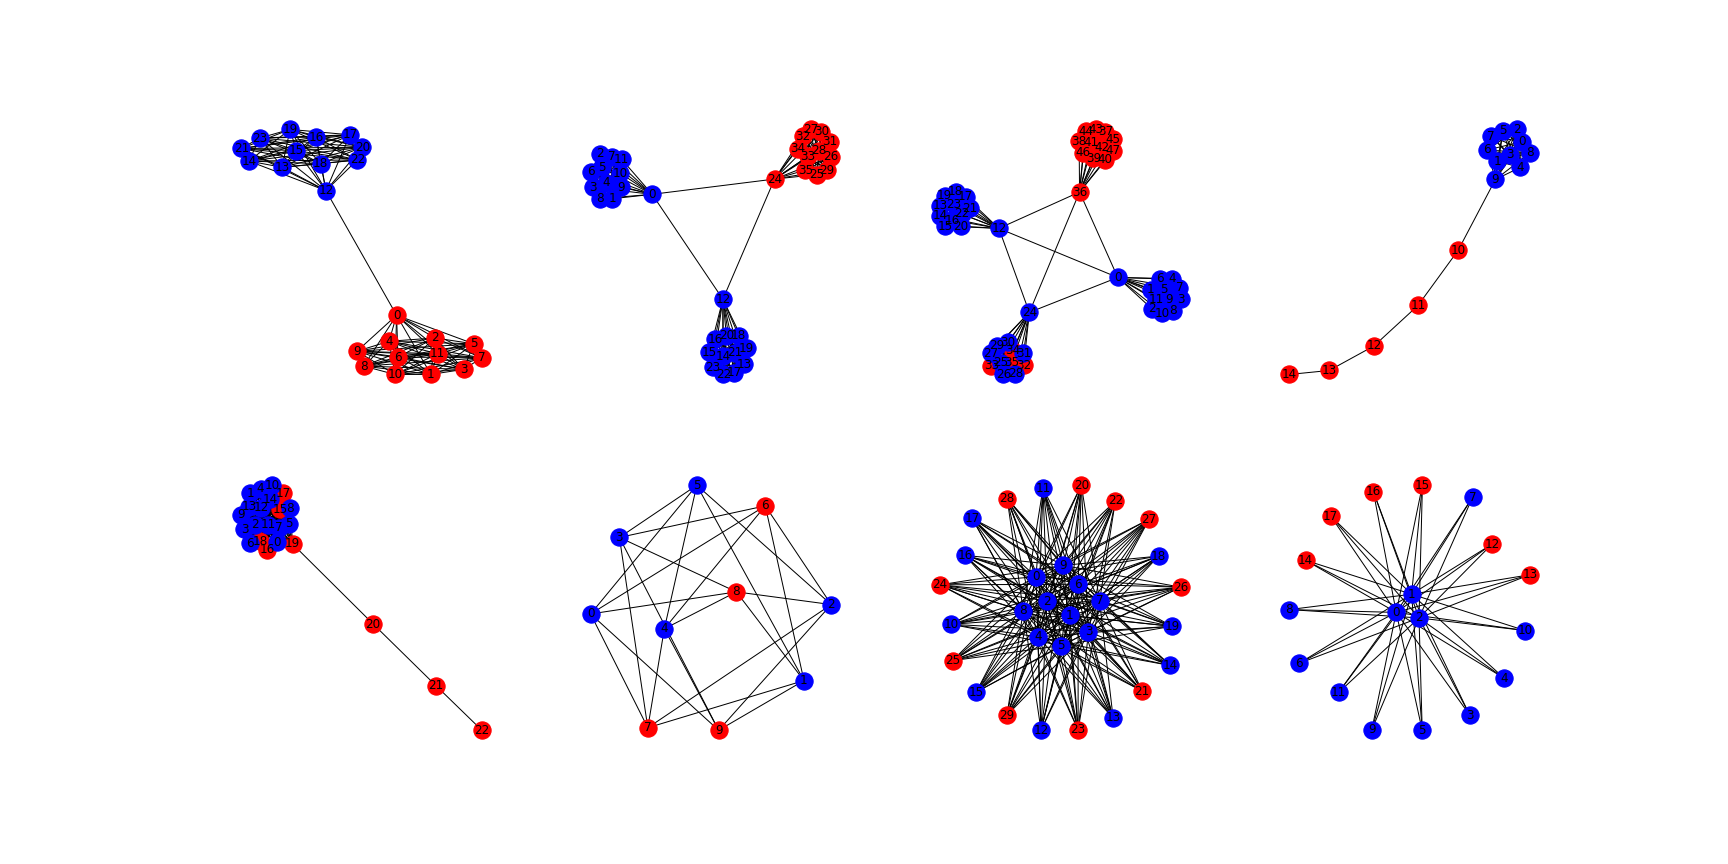
\includegraphics[width=180mm]{test.png}
    \caption{Тестовые примеры работы алгоритма Лейтона-Рао}
    \label{FigExample}
\end{figure}

Как видно из примеров на "хорошо разделяемых" графах алгоритм выдает отличные результаты, что говорит о правильной реализации алгоритма. Также чем больше вершин в графе, тем более красивые и "визуально правильные" результаты получаются.

\newpage

%%%%%%%%%%%%%%%%%%%%%%%%%%%%%%%%%%%%%%%%%%%%%%%%%%%%%%%%%%%%%%%%%%%%%%%%%%
\section{Литература}
%%%%%%%%%%%%%%%%%%%%%%%%%%%%%%%%%%%%%%%%%%%%%%%%%%%%%%%%%%%%%%%%%%%%%%%%%%

\begin{itemize}
\item
    Tom Leighton and Satish Rao. 1999. Multicommodity Max-Flow Min-Cut Theorems and Their Use In Designing Approximation Algorithms
\end{itemize}


\nocite{bishop06pattern,hastie09elements,kolmogorov87information,zhuravlev78prob33,langley00crafting,blake98uci}

\def\BibUrl#1.{\\{\footnotesize\tt\def~{\char126} http://#1}}
\def\BibAnnote#1.{}

% Автоматическая генерация библиографии по библиографической базе
\bibliographystyle{gost71s}
\bibliography{MachLearn}

\end{document}

